\section{Results and Discussion}
\label{sec:Results_and_Discussion}
This section contains lists of all important results and summarizes the most important things.

\subsection{Ultrasound Speed $c$}
\label{subsec:Ultrasound_Speed}
The following figures \ref{fig:results_ultrasound_speed} and \ref{fig:results_metals} show a graphical comparison between the calculated and the litearture values for the sound velocity.

\begin{figure}[H]
	\centering
	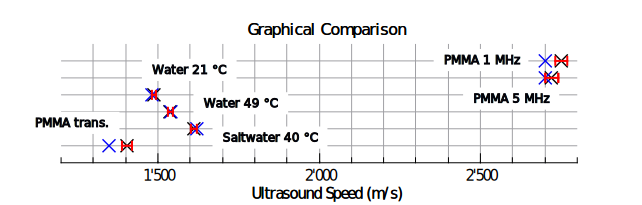
\includegraphics[scale=0.94]{results_ultrasound_speed}
	\caption{Graphical comparison between the calculated values (black cross with red uncertainty bar) and their respective literature values (blue cross). Especially the ultrasound speed of water is extremely close to the litearature value. The calculated sound velocities in PMMA at an oscillation frequency of 1 MHz are off by quite a bit (both logitudinal and transversal).}
	\label{fig:results_ultrasound_speed}
\end{figure}

\begin{figure}[H]
	\centering
	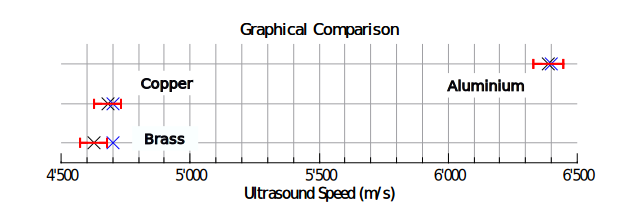
\includegraphics[scale=0.94]{results_metals}
	\caption{Graphical comparison of the three different metals aluminium, copper and brass. They are compared separately because their sound velocity is in a different range. This would have stretched out figure \ref{fig:results_ultrasound_speed} above and thus would have made it less readable. The literature values of the sound velocity (blue) in aluminium and copper lie inside the error bars of the respective metals.}
	\label{fig:results_metals}
\end{figure}

Table \ref{tab:Ultrasound_Speed} shows all calculated sound velocities and their respective literature values in one table.

\begin{table}[H]
	\centering
	\renewcommand{\arraystretch}{1.1}
	\begin{tabular}{|l|c|c|c|}
		\cline{2-4}
		\multicolumn{1}{c|}{} & $\boldsymbol{c}$ \textbf{@ 1 MHz} & $\boldsymbol{c}$ \textbf{@ 5 MHz} & \textbf{Litearture} \\
		\multicolumn{1}{c|}{} & in m/s & in m/s & in m/s \\
		\hline
		\textbf{PMMA} & $(2751\pm 19)$ & $(2721\pm 21)$ & $\approx 2700$ \\
		\hline
		\textbf{Aluminium} & - & $(6387\pm 59)$ & $\approx 6400$ \\
		\hline
		\textbf{Copper} & - & $(4680\pm 53)$ & $\approx 4700$ \\
		\hline
		\textbf{Brass} & - & $(4627\pm 52)$ & $\approx 4700$ \\
		\hline
		\textbf{Water 21 \textdegree C} & - & $(1488\pm 7)$ & $\approx 1483$ \\
		\hline
		\textbf{Water 49 \textdegree C} & - & $(1538\pm 8)$ & $\approx 1540$ \\
		\hline
		\textbf{Saltwater 40 \textdegree C} & - & $(1612\pm 10)$ & $\approx 1620$ \\
		\hline
		\textbf{PMMA trans.} & $(1405\pm 15)$ & - & $\approx 1350$ \\
		\hline
	\end{tabular}
	\caption{Summary of all calculated sound velocities and their respective literature values for the oscillation frequencies 1 MHz and 5 MHz.}
	\label{tab:Ultrasound_Speed}
\end{table}

% -----------------------------------------------------------------------------------------
\subsection{Attenuation Coefficient $\mu$}
\label{subsec:Attenuation_Coefficient}
The following figure \ref{fig:results_absorption} shows a graphical comparison between the two calculated attenuation coefficients and their uncertainties.

\begin{figure}[H]
	\centering
	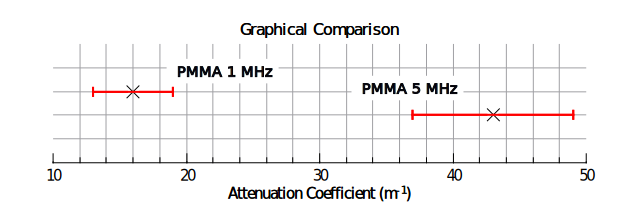
\includegraphics[scale=0.94]{results_absorption}
	\caption{Graphical comparison between the calculated values (black cross with red uncertainty bar) and their respective literature values (blue cross). The calculated attenuatin coefficient for PMMA at a frequency of 5 MHz is very imprecise. This is due to the fact, that the amplitude values are approaching 0 very fast. Thus, it is hard to get accurate readings (see figure \ref{fig:measuring_procedure}).}
	\label{fig:results_absorption}
\end{figure}

Table \ref{tab:Attenuation_Coefficient} shows the values of the calculated attenuation coefficients.

\begin{table}[H]
	\centering
	\renewcommand{\arraystretch}{1.1}
	\begin{tabular}{|l|c|c|}
		\cline{2-3}
		\multicolumn{1}{c|}{} & $\boldsymbol{\mu}$ \textbf{@ 1 MHz} & $\boldsymbol{\mu}$ \textbf{@ 5 MHz} \\
		\multicolumn{1}{c|}{} & in m$^{-1}$ & in m$^{-1}$ \\
		\hline
		\textbf{PMMA} & $(16\pm 3)$ & $(43\pm 6)$ \\
		\hline
	\end{tabular}
	\caption{Summary of the calculated attenuation coefficients for the oscillation frequencies 1 MHz and 5 MHz.}
	\label{tab:Attenuation_Coefficient}
\end{table}
